\begin{frame}[plain]
  \begin{tikzpicture}[remember picture,overlay]
    \node[at=(current page.center)] {
      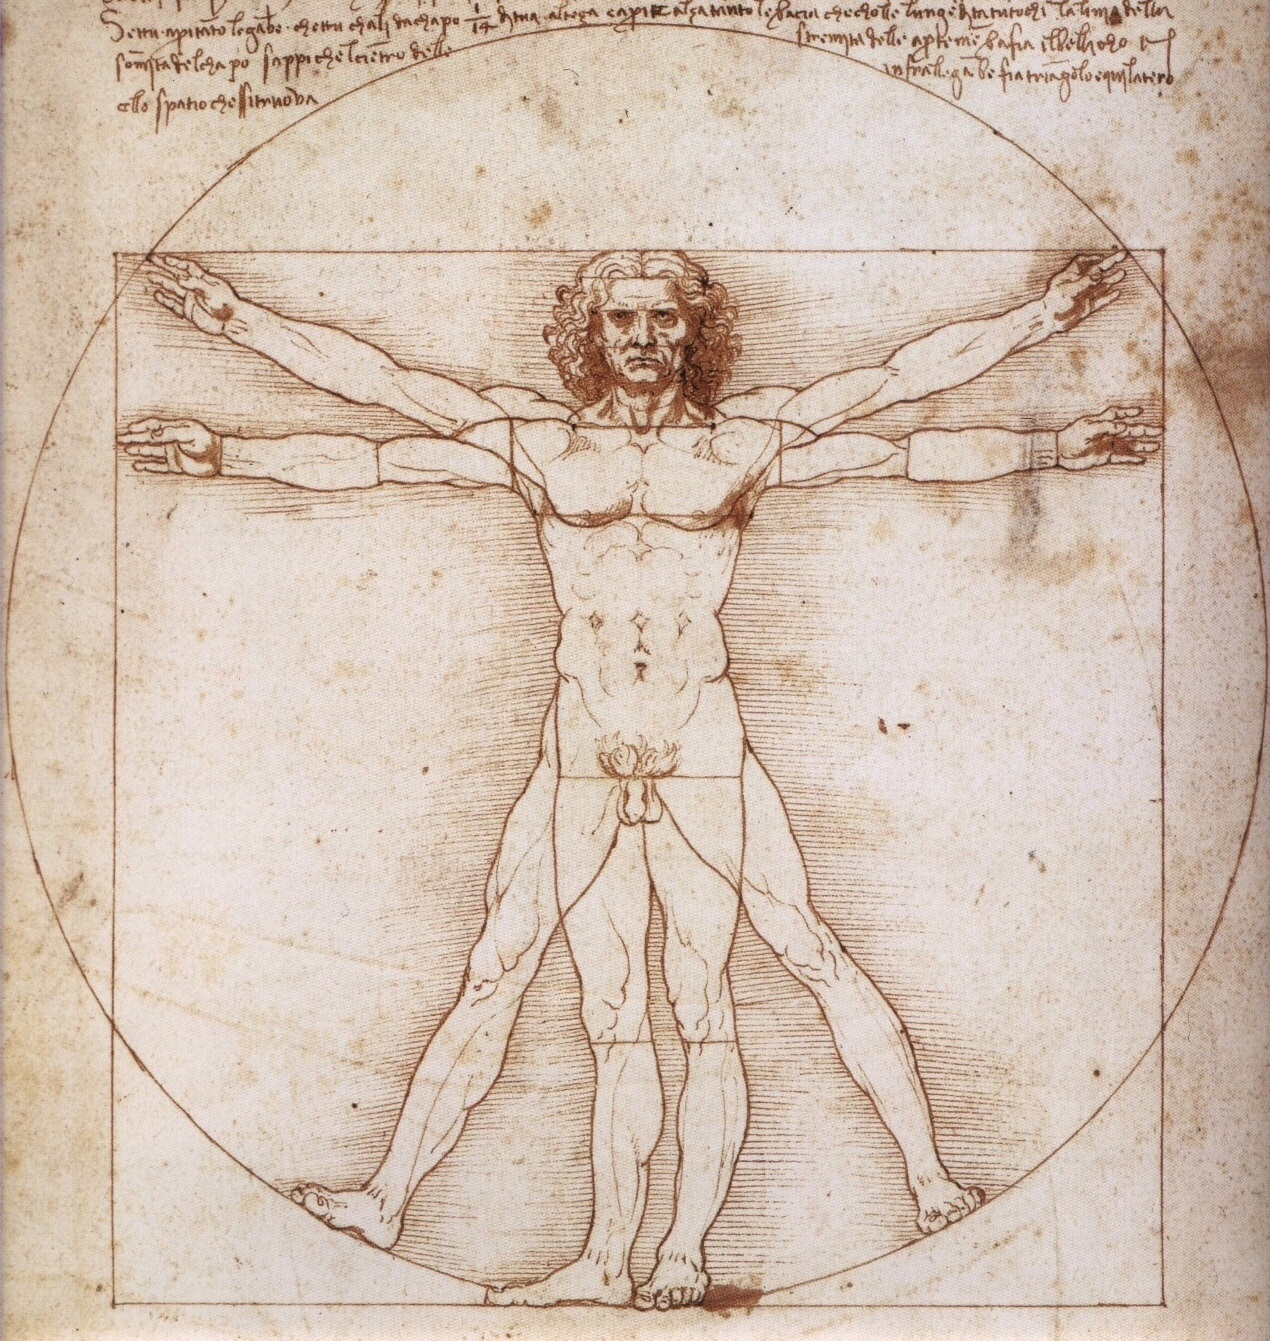
\includegraphics[width=\paperwidth]{uomo_vitruviano.jpg}
    };
  \end{tikzpicture}
\end{frame}

\section{Part-Based Model for Object Detection}

\begin{frame}{Part-Based Model}
  \metroset{block=fill}
  \begin{block}{Idea}
    An object is made of a set of specific sub-blocks.
  \end{block}
  \pause
  \begin{block}{Pictorial structure}
    Pictorial structures represent objects by a collection of parts arranged in
    a deformable configuration.
  \end{block}
\end{frame}


\begin{frame}{Pictorial Structures}
  \centering
  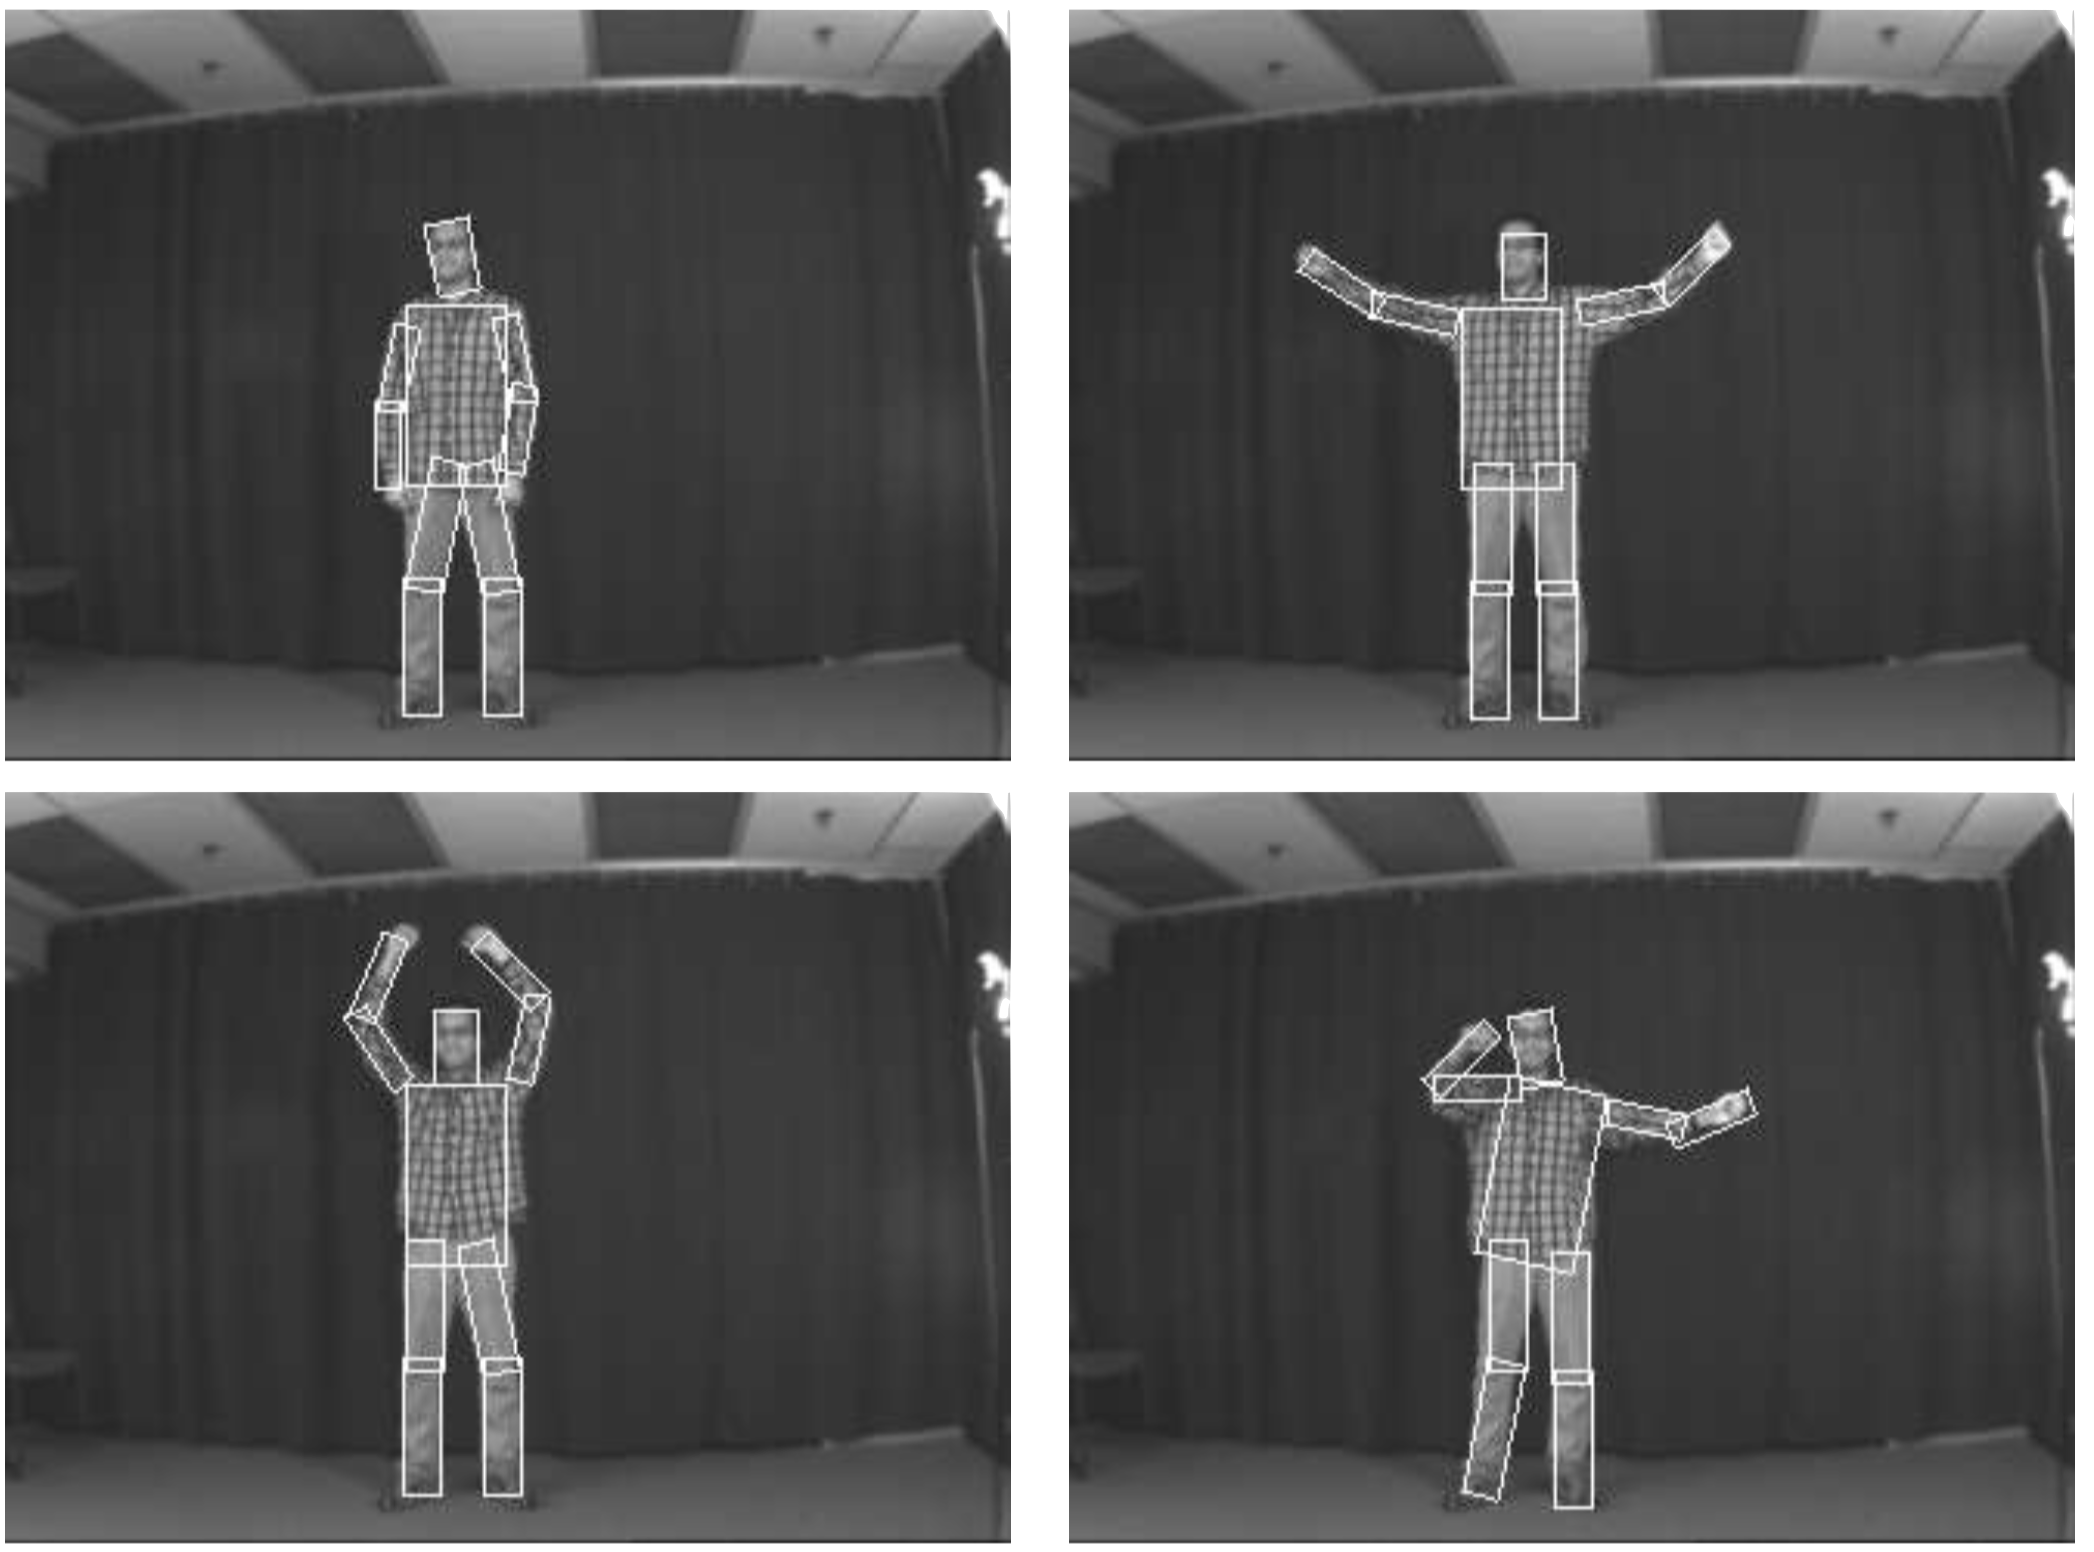
\includegraphics[width=.95\textwidth]{pictorial_structures.png}
\end{frame}

\begin{frame}{Part-based Models}
  \metroset{block=fill}
  \begin{exampleblock}{Idea}
    The idea is to give a \textbf{score} for each part of the model (e.g. for
    humans could be arm, chest, legs, face, \dots).
  \end{exampleblock}
  \pause
  \begin{alertblock}{Starting point}
    We would like to define a score at different positions and scales in an image.
    This is done using a feature pyramid which specifies a feature map for a finite
    number of scales in a fixed range.
  \end{alertblock}
\end{frame}

\begin{frame}{Scores}
  Given a model based on $n$ parts, generally:
  \begin{equation*}
  \mbox{score}(x_0,y_0) = R_{l_0}(x_0, y_0) + \sum_{i=1}^nD_{l_0-\lambda}(2(x_0,y_0)+v_i)+b
  \end{equation*}
  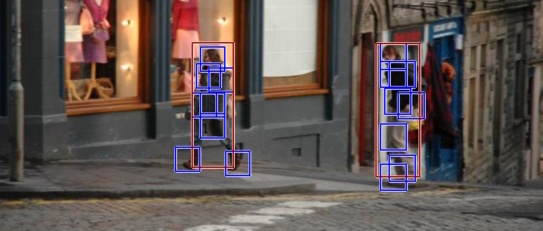
\includegraphics[width=\textwidth]{part_based_example.jpg}
\end{frame}
